\documentclass[main.tex]{subfiles}
\begin{document}
\subsection{Find Multiplication table for a group $G=\{3$ elements$\}$ and prove that it is unique.}
Consider the group of three elements $G=\{e,a,b\}$. By the four group axioms the only table we may have is
\[
    \begin{tabular}{>{$}l<{$}|*{3}{>{$}l<{$}}}
    ~   & e   & a   & b   \\
    \hline\vrule height 12pt width 0pt
    e   & e   & a   & b  \\
    a   & a   & b & e     \\
    b & b & e   & a     \\

    \end{tabular} 
\]
because of closure we must have $aa=a^2=b$, $ab=e$ and $bb=a$. Now suppose the table is not unique, to satisfy closure the only other property we can think of would be $aa=e$ and then $aab=b$ and $a=a^{-1}$ $\implies aaa^{-1}=ba$, but then $a=ba\implies b=e$ and thus the group has only two elements and thus the multiplication table for a group with three elements is unique.
\subsection{Find all unique multiplication tables for groups for four elements.}
For $G=\{e,a,b,c\}$ there are two unique multiplication tables. First write out
\[
    \begin{tabular}{>{$}l<{$}|*{4}{>{$}l<{$}}}
    ~   & e   & a   & b & c    \\
    \hline\vrule height 12pt width 0pt
    e   & e   & a   & b   & c  \\
    a   & a   & a^2 & ab  & ac  \\
    b   & b   & ba  & b^2 & bc  \\
    c   & c   & ca  & cb  & c^2  \\
    \end{tabular} 
\]
The first possible table which obeys the four group axoims begins with $aa=b$ and $bb=aaaa=e$, $c^2=(ab)^2=a^2a^4=a^2$, $ac=e$ the table is
\[
    \begin{tabular}{>{$}l<{$}|*{4}{>{$}l<{$}}}
    ~   & e   & a   & b & c    \\
    \hline\vrule height 12pt width 0pt
    e   & e   & a  & b  & c  \\
    a   & a   & b  & c  & e  \\
    b   & b   & c  & e  & a  \\
    c   & c   & e  & a  & b  \\
    \end{tabular} 
\]
This table describes the group $\mathbb{Z}_4$, the additive group of integers modulo $4$.

The other possibility is
\[
    \begin{tabular}{>{$}l<{$}|*{4}{>{$}l<{$}}}
    ~   & e   & a   & b & c    \\
    \hline\vrule height 12pt width 0pt
    e   & e   & a  & b  & c  \\
    a   & a   & e  & c  & b  \\
    b   & b   & c  & e  & a  \\
    c   & c   & b  & a  & e  \\
    \end{tabular} 
\]
This table descibes the group $\mathbb{Z}_2\times\mathbb{Z}_2$.
\subsection{ Show that the defining representation of $S_n$ is reducible}
\subsection{ Suppose $D_1$, $D_2$ equivalent irreps of a group $G$ $\st$ $D_2(g)=SD_1(g)S^{-1}\forall g\in G$, what can we say about an operator $A$ that satisfies $AD_1(g)=D_2(g)A$?}
$AD_1(g)=D_2(g)A=SD_1(g)S^{-1}A$ then $S^{-1}AD_1{g}=D_1(g)S^{-1}A$. Then, by Schur's lemma $S^{-1}A\propto\mathbb{I}$ so that $A\propto S$ but because we are always free to rescale the similarity transformation by an arbitrary constant $A=S$.
\subsection{Find the symmetries of the regular tetrahedron invariant. Find the conjugacy classes and the characters of the irreps of the group}

\begin{figure}[H] 
\centering
  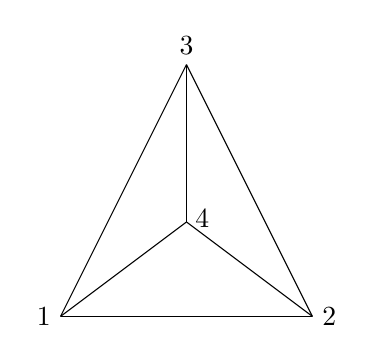
\begin{tikzpicture}[scale=.4]
    \draw (0,0) -- (0,5);
    \draw (-4,-3) -- (0,0);
    \draw (4,-3) -- (0,0);
    \draw (-4,-3) -- (4,-3);
    \draw (0,5) -- (4,-3);
    \draw (0,5) -- (-4,-3);
    \node [left] at (-4,-3) {$1$};
    \node [right] at (4,-3) {$2$};
    \node [above] at (0,5) {$3$};
    \node at (0.5,0.1) {$4$};
  \end{tikzpicture}
\end{figure}
The regular tetrahedron symmetries are given by the $4!=24$ ways we can rearrange the labels $1,2,3,4$
Firstly, the rotations are 
\begin{align}
(1,2,3,4)&\rightarrow(1,2,3,4) = e\\
(1,2,3,4)&\rightarrow(2,3,1,4)\\
(1,2,3,4)&\rightarrow(3,1,2,4)\\
(1,2,3,4)&\rightarrow(1,4,2,3)\\
(1,2,3,4)&\rightarrow(1,3,4,2)\\
(1,2,3,4)&\rightarrow(4,2,1,3)\\
(1,2,3,4)&\rightarrow(3,2,4,1)\\
(1,2,3,4)&\rightarrow(4,1,3,2)\\
(1,2,3,4)&\rightarrow(2,4,3,1)\\
(1,2,3,4)&\rightarrow(2,1,4,3)\\
(1,2,3,4)&\rightarrow(3,2,1,4)\\
(1,2,3,4)&\rightarrow(4,3,2,1)
\end{align}
The odd permutations are 
\begin{align}
(1,2,3,4)&\rightarrow(2,1,3,4)\\
(1,2,3,4)&\rightarrow(3,2,1,4)\\
(1,2,3,4)&\rightarrow(4,2,3,1)\\
(1,2,3,4)&\rightarrow(1,3,2,4)\\
(1,2,3,4)&\rightarrow(1,4,3,2)\\
(1,2,3,4)&\rightarrow(1,2,4,3)\\
(1,2,3,4)&\rightarrow(4,3,1,2)\\
(1,2,3,4)&\rightarrow(2,3,4,1)\\
(1,2,3,4)&\rightarrow(3,4,1,2)\\
(1,2,3,4)&\rightarrow(3,1,4,2)\\
(1,2,3,4)&\rightarrow(3,4,2,1)\\
(1,2,3,4)&\rightarrow(3,2,4,1)
\end{align}
\subsection{Analyse the normal modes of the system of four blocks sliding on a frictionless plane connected by springs.}
\end{document}